In diesem Kapitel werden die gängigen 2FA-Verfahren im Kontext von 
Online-Anwendungen vorgestellt. Des Weiteren werden auch die Vor- und Nachteile dieser Verfahren beleuchtet. 
Leider gibt es nur wenige Studien zu 2FA-Verfahren, die insbesondere verlässliche 
Zeitmessungen bzgl. der Nutzerinteraktionen bieten. Grundlegende Erkenntnisse liefert die Studie 
von \textcite{Reese}. Hier wurden verschiedene 
2FA-Verfahren hinsichtlich ihrer Nutzerfreundlichkeit und ihres Zeitaufwandes 
untersucht. Es wurden die gängigsten Verfahren untersucht:
\begin{itemize}
    \item Vorab generierte Codes
    \item Push-Benachrichtigungen (Authy)
    \item Einmalpasswort per SMS
    \item Zeitbasiertes Einmalpasswort (Google Authenticator)
    \item Universal Second Factor Security Keys (USB-Gerät YubiKey)
    \item Nur Passwort ohne zweiten Faktor (als Kontrollgruppe)
\end{itemize}
Dabei gab es sechs Studiengruppen mit je 12 Teilnehmern. Jede Studiengruppe hat eine 
der sechs untersuchten Authentisierungsverfahren eingerichtet und in einer 
zweiwöchigen Phase genutzt, um sich täglich bei einem Webdienst anzumelden. Es 
wurde die benötigte Zeit für die Einrichtung des Verfahrens sowie für die Eingabe bzw. 
Bestätigung des zweiten Faktors serverseitig gemessen. 
Neben qualitativen Ergebnissen aus Interviews wurde unter anderem auch die Benutzbarkeit mit der System 
Usability Scale (SUS) ermittelt.
\\\\
In der Studie gibt es pro Studiengruppe (also pro Verfahren) eine Zeitmessung und 
eine SUS-Bewertung für den Authentisierungsprozess. Die Ergebnisse sind in Abb. \ref{fig: reese sus} und Abb. \ref{fig: reese zeiten} dargestellt. Die zugehörigen Tabellen für die exakten Werte befinden sich im Anhang \ref{anh: reese}.
\\
\begin{figure}
    \begin{minipage}[b]{.48\textwidth}
        \centering
        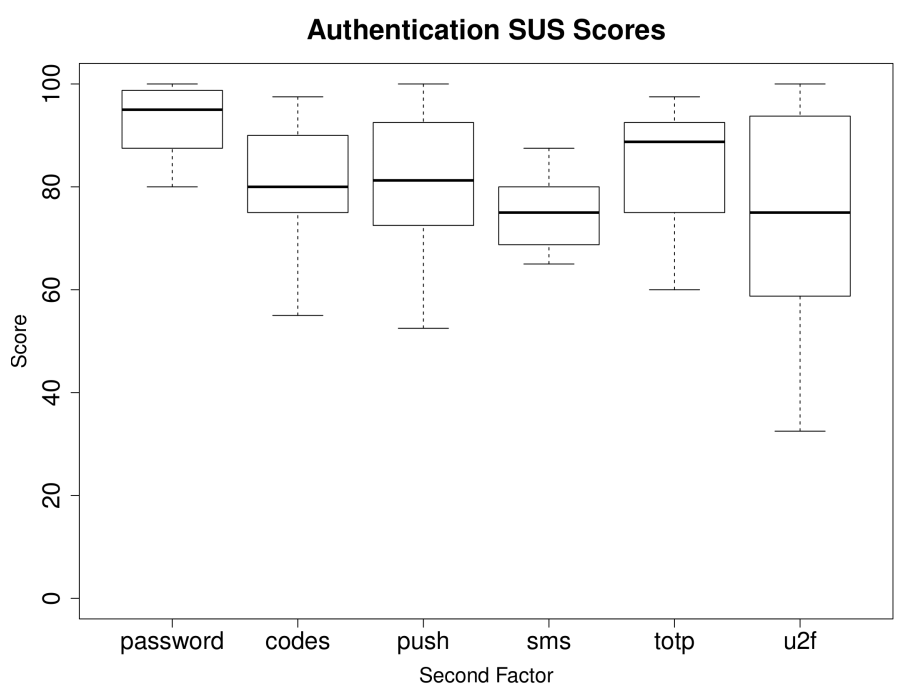
\includegraphics[width=1\linewidth]{figures/susAuth.png}
        \caption[SUS-Bewertung für die Authentisierung mit verschiedenen 2FA-Verfahren]{SUS-Bewertung für die Authentisierung mit verschiedenen 2FA-Verfahren, entnommen aus \autocite[363]{Reese}}
        \label{fig: reese sus}
    \end{minipage}
    \hfill
    \begin{minipage}[b]{.48\textwidth}
        \centering
        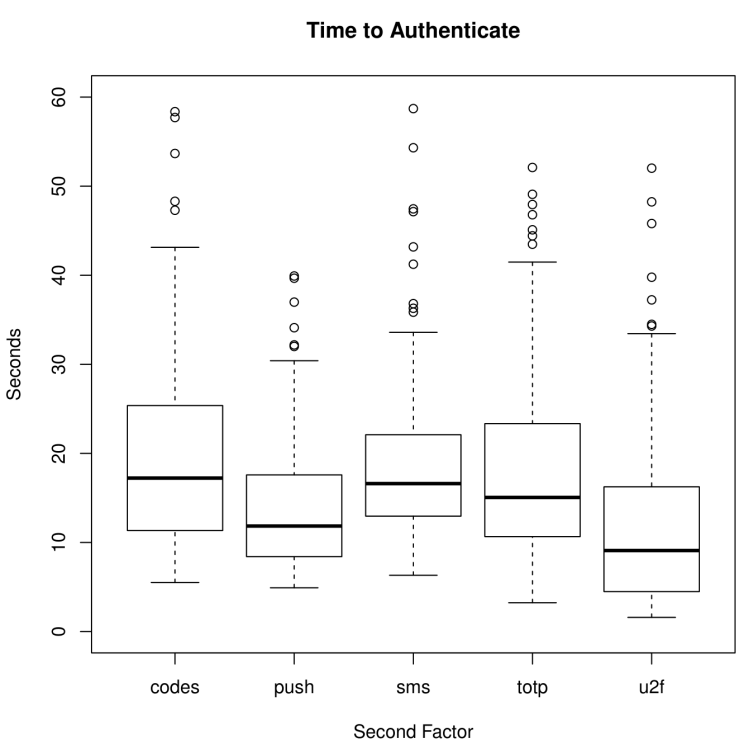
\includegraphics[width=1\linewidth]{figures/timeToAuth.png}
        \caption[Benötigte Zeit für die Authentisierung mit verschiedenen 2FA-Verfahren]{Benötigte Zeit für die Authentisierung mit verschiedenen 2FA-Verfahren, entnommen aus \autocite[362]{Reese}}
        \label{fig: reese zeiten}
    \end{minipage}
\end{figure}

Im Verlauf dieses Kapitels werden die Ergebnisse genutzt, um die vorgestellten 
2FA-Verfahren bzgl. ihrer Nutzerfreundlichkeit und ihres Zeitaufwandes einzuordnen.
